\chapter{Izpeljava gibanja sonde relativno na magnet ob nepravilni montaži}

Nepravilna montaža bo vplivala na  Hallove sondi simulacijskega modela enako. Vpliv izmika senzorja in magneta, na relativno gibnaje sonde nad magnetom bo prikazano na eni sondi.

Izmik sredine senzorja iz osi vrtenja bo med spreminjanjem dejanskega kota zasuka statičen, njegova lokacija se nebo spreminjala na os vrtenja. Ta izmik je poimenovan statična ekscentričnost.

Ob izmiku magneta iz osi vrtenja se pojavi opletanje magneta. Lokacija središča magneta se spreminja glede na določen zasuk magneta. Opletanje magneta je poimenovano dinamična ekscentričnost.
\section{Definicija koordinatnega sistema}
Naj bo definiran kartezični koordinatni sistem, z v izhodišču postavljenim radialno polariziranim magnetom ($S_m(0, 0)$). V izhodišču se nahaja tudi os vrtenja ($S_r(0, 0)$). Na poljubno točko $H(x_0,y_0)$, vendar ne v
izhodišče je postavljena Hall-ova sonda (slika \ref{fig:def_kks}).
\begin{figure}[!ht]
	\centering
	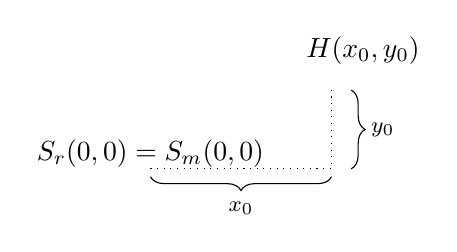
\begin{tikzpicture}
	\magnet {0} {0} {0}{ }{1};
	\hall {2.3}{1} {0};
	\draw [decorate,decoration={brace,amplitude=5pt,mirror},xshift= 0pt,yshift=0pt]
	(2.55,0) -- (2.55,1) node [black,midway,xshift= 0.4cm] 
	{\footnotesize $y_0$};
	\draw [decorate,decoration={brace,amplitude=5pt,mirror},xshift= 0pt,yshift=0pt]
	(0,-0.1) -- (2.3,-0.1) node [black,midway,yshift= -0.4cm] 
	{\footnotesize $x_0$};
	\draw[dotted](0,0)--(2.3,0)--(2.3,1) node[yshift = 0.5cm, xshift = 0.4 cm] {$H(x_0,y_0)$};
	\node at (0,0.2) {$S_r(0, 0)=S_m(0, 0)$};
	\end{tikzpicture}
	\caption{Definicija koordinatnega sistema z magnetom in Hall-ovo sondo}
	\label{fig:def_kks}
\end{figure}

Z zasukom magneta za kot $\theta$, se lokacija sonde glede na magnet spremeni. Nova lokacija sonde glede na magnet je enaka, če se namesto magnet, zavrti sondo za kot $-\theta$ . Nova lokacija
sonde glede na magnet je v točki  $(x, y)$. Novo lokacijo sonde glede na magnet v odvisnosti od zasuka magneta za kot $\theta$, opiše enačba (\ref{equ:rotacija_hall}).
\begin{equation}
\label{equ:rotacija_hall}
\begin{bmatrix} x\\y \end{bmatrix}=
\begin{bmatrix} \cos(-\theta)&-\sin(-\theta)\\\sin(-\theta)&\cos(-\theta) \end{bmatrix}
\begin{bmatrix} x_0\\y_0 \end{bmatrix}
\end{equation}

Argument rotacijske matrike je $-\theta$. Z upoštevanjem lihosti funkcije sinus in sodosti funkcije kosinus\cite{Matematika1}, se (\ref{equ:rotacija_hall}) poenostavi v:
\begin{equation}
%\label{equ:rotacija_hall_simplify}
\begin{bmatrix} x\\y \end{bmatrix}=
\begin{bmatrix} \cos(\theta)&\sin(\theta)\\-\sin(\theta)&\cos(\theta) \end{bmatrix}
\begin{bmatrix} x_0\\y_0 \end{bmatrix}
\end{equation}
\begin{figure}[!ht]
    \begin{subfigure}[b]{0.5\textwidth}
	\centering
		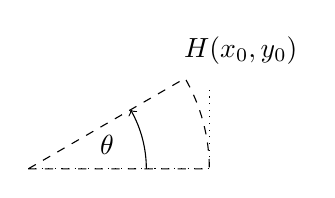
\begin{tikzpicture}
		[scale=1, every node/.style={scale=1}]
				\magnet {0} {0} {30}{}{1}
				\hall {2.3}{0+1} {0};
				\draw[dotted](0,0)--(2.3,0)--(2.3,1) node[yshift = 0.5cm, xshift = 0.4 cm] {$H(x_0,y_0)$};
				\draw [dashed](0,0)--(2.3,0) arc (0:30:2.3)--(0,0);
				\node at(1,0.3){$\theta$};
                \draw [->] (1.5,0) arc (0:30:1.5);
		\end{tikzpicture}
	\caption{Zasukan magnet za kot $\mathrm{\theta}$}
	\label{subfig:zasuk_magnet}
\end{subfigure}
\begin{subfigure}[b]{0.5\textwidth}
	\centering
		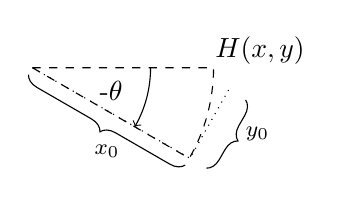
\begin{tikzpicture}[scale=1, every node/.style={scale=1}]		
				\magnet {0} {0} {0}{}{1}
				\hall {2.4919}{-0.2839} {-30};
				\draw [dashed](0,0)--(2.3,0) arc (0:-30:2.3)--(0,0);
				\node at(1,-0.3){-$\theta$};
                \draw [->] (1.5,0) arc (0:-30:1.5);
                
                \draw[dotted](0,0)--(2,-1.15)--(2.49,-0.2839) node[yshift = 0.5cm, xshift = 0.4cm] {$H(x,y)$};
                \draw [decorate,decoration={brace,amplitude=5pt,mirror},xshift= 0pt,yshift=0pt]
                (2.2084,-1.275) -- (2.7084,-0.40897) node [black,midway,xshift= 0.4cm] 
                {\footnotesize $y_0$};
                \draw [decorate,decoration={brace,amplitude=5pt,mirror},xshift= 0pt,yshift=0pt]
                (-0.05,-0.086603) -- (1.9419,-1.2366) node [black,midway,yshift= -0.4cm] 
                {\footnotesize $x_0$}; 
		\end{tikzpicture}
	
	\caption{Zasukan senzor za kot $\mathrm{-\theta}$}
	\label{subfig:zasuk_hall}
\end{subfigure}
\caption{Sprememba položaja glede na magnet ob rotaciji}
\label{fig:zasuk_magneta}
\end{figure}
\section{Izpeljava gibanja lokacije Hallove sonde na magnet pri dinamični ekscentričnosti}
Magnet je postavljen v izhodišce koordinatnega sistema $S_m(0,0)$, kjer je tudi os vrtenja $S_r(0,0)$. Dinamična ekscentričnost povzroči premik središča magneta v točko $S_{m1}(\Delta x_d,\Delta y_d)$ (Slika \ref{fig:def_din_eks}).
Os vrtenja je ostaja v izhodišču koordinatnega sistema. Središce magneta $S_{m1}(\Delta x_d,\Delta y_d)$ ob rotaciji opiše okoli osi vrtenja krožnico z radijem $\sqrt{\Delta x_d^2+\Delta y_d^2}$.% (\ref{equ:rotacija_hall_din_sonda}).
\begin{figure}[!ht]
	\centering
	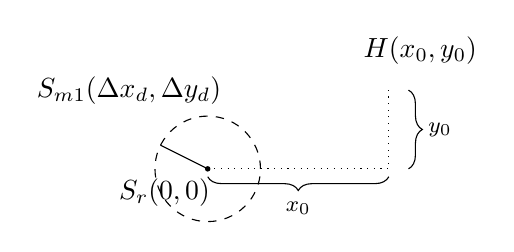
\begin{tikzpicture}
		\magnet {-0.6} {0.3} {0}{ }{1};
		\hall {2.3}{1} {0};
		\kks{3}
		\draw [dashed]  (0,0) circle (0.67);
		\draw (0,0)--(-0.6,0.3);
		\fill (0,0) circle [radius=1pt];
		\node at (-0.55,-0.3){$S_r(0,0)$};
		\node at(-1,1){$S_{m1}(\Delta x_d,\Delta y_d)$};
		\draw [decorate,decoration={brace,amplitude=5pt,mirror},xshift= 0pt,yshift=0pt]
		(2.55,0) -- (2.55,1) node [black,midway,xshift= 0.4cm] 
		{\footnotesize $y_0$};
		\draw [decorate,decoration={brace,amplitude=5pt,mirror},xshift= 0pt,yshift=0pt]
		(0,-0.1) -- (2.3,-0.1) node [black,midway,yshift= -0.4cm] 
		{\footnotesize $x_0$};
		\draw[dotted](0,0)--(2.3,0)--(2.3,1) node[yshift = 0.5cm, xshift = 0.4 cm] {$H(x_0,y_0)$};
	\end{tikzpicture}
	\caption{Definicije dinamične ekscentričnosti}
	\label{fig:def_din_eks}
\end{figure}

Naj ostane magnet v izhodišču $S_m(0,0)$ in naj se spremeni lokacija Hallove sonde in os vrtnja za $(-\Delta x_d,-\Delta y_d)$ (Slika \ref{fig:def_din_eksbac}). Sondo se tako kot v prejšnjem poglavju zavrti 
v nasprotno stran okoli osi vrtenja. Os vrtenja je v točki $(-\Delta x_d,-\Delta y_d)$. Sonda se giblje po krožnici s središčem v točki $(-\Delta x_d,-\Delta y_d)$. Spreminjanje lokacije sonde glede na 
magnet opiše (\ref{equ:rotacija_hall_din})
\begin{equation}
\label{equ:rotacija_hall_din}
\begin{bmatrix} x\\y \end{bmatrix}=
\begin{bmatrix} \cos(\theta)&\sin(\theta)\\-\sin(\theta)&\cos(\theta) \end{bmatrix}
\begin{bmatrix} x_0\\y_0 \end{bmatrix}
-
\begin{bmatrix} \Delta x_d\\\Delta y_d \end{bmatrix}
\end{equation}
\begin{figure}[!ht]
	\centering
	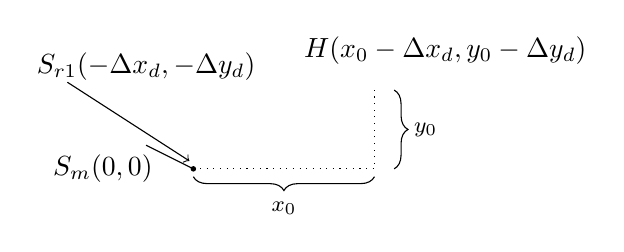
\begin{tikzpicture}
	\magnet {0} {0} {0}{ }{1};
	\hall {2.3+0.6}{1-0.3} {0};
	\kks{3}
	\draw (0,0)--(0.6,-0.3);
	\fill (0.6, -0.3) circle [radius=1pt];
	\node at (-0.55,-0.3){$S_m(0,0)$};
	\node at(0,1){$S_{r1}(-\Delta x_d,-\Delta y_d)$};
	\draw [->](-1,0.8)--(0.55,-0.2);
	\draw [decorate,decoration={brace,amplitude=5pt,mirror},xshift= 0pt,yshift=0pt]
	(2.55+0.6,0-0.3) -- (2.55+.6,1-.3) node [black,midway,xshift= 0.4cm] 
	{\footnotesize $y_0$};
	\draw [decorate,decoration={brace,amplitude=5pt,mirror},xshift= 0pt,yshift=0pt]
	(0+.6,-0.1-.3) -- (2.3+.6,-0.1-.3) node [black,midway,yshift= -0.4cm] 
	{\footnotesize $x_0$};
	\draw[dotted](0+.6,0-.3)--(2.3+.6,0-.3)--(2.3+.6,1-.3) node[yshift = 0.5cm, xshift = 0.9 cm] {$H(x_0-\Delta x_d,y_0-\Delta y_d)$};
	\end{tikzpicture}
	\caption{Premik osi vrtenja in sonde za velikost dinamične ekscentričnosti}
	\label{fig:def_din_eksbac}
\end{figure}
\section{Izpeljava gibanja lokacije Hall-ove sonde na magnet pri statični ekscentričnosti}
Statična ekscentričnost se pojavi, ob izmiku Hallove sonde iz njene osnovne lege v  $H_1(x_0+\Delta x_s, y_0+\Delta y_s)$. Z zasukom magneta je razdalja med sondo in osjo vrtenja konstantna.
Z miselnim obratom vrtenja sonde v nasprotni smeri se gibanje sonde izrazi kot gibanje po krožnici z novim radijem $\sqrt{(x_0+\Delta x_s)^2+(y_0+\Delta y_s)^2}$ (\ref{equ:rotacija_hall_stat}).
\begin{figure}[!ht]
	%\centering
	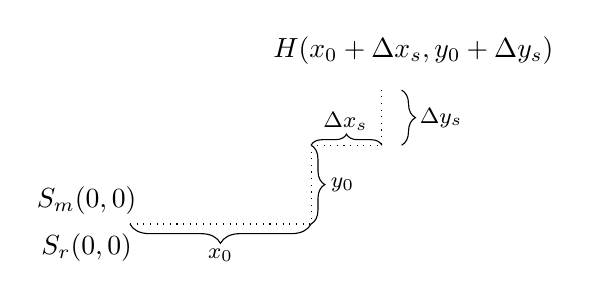
\begin{tikzpicture}
	\kks{3}
	\magnet {0} {0} {0}{}{1};
	\hall {2.3+0.9}{1+0.7} {0};
	\node at (-0.55,-0.3){$S_r(0,0)$};
	\node at(-0.55,0.3){$S_{m}(0,0)$};
	\draw [decorate,decoration={brace,amplitude=5pt,mirror},xshift= 0pt,yshift=0pt]
	(2.3,0) -- (2.3,1) node [black,midway,xshift= 0.4cm] 
	{\footnotesize $y_0$};
	\draw [decorate,decoration={brace,amplitude=7pt,mirror},xshift= 0pt,yshift=0pt]
	(0,0) -- (2.3,0) node [black,midway,yshift= -0.4cm] 
	{\footnotesize $x_0$};
	\draw[dotted](0,0)--(2.3,0)--(2.3,1)--(2.3+0.9,1)--(2.3+0.9,1+0.7) node[yshift = 0.5cm, xshift = 0.4 cm] {$H(x_0 + \Delta x_s ,y_0+ \Delta y_s)$};
	\draw [decorate,decoration={brace,amplitude=4pt},xshift= 0pt,yshift=0pt]
	(2.3,1) -- (2.3+0.9,1) node [black,midway,xshift = -0.4 ,yshift= 0.3cm] 
	{\footnotesize $\Delta x_s$};
	\draw [decorate,decoration={brace,amplitude=5pt,mirror},xshift= 0pt,yshift=0pt]
	(2.3+0.9+0.25,1)--(2.3+0.9+0.25,1+0.7) node [black,midway,xshift= 0.5cm] 
	{\footnotesize $\Delta y_s$};
	\end{tikzpicture}
	\caption{Definicije statične ekscentričnosti}
	\label{fig:def_sta_eks}
\end{figure}
Novo lokacijo sonde glede na magnet opiše (\ref{equ:rotacija_hall_stat}). Ob povzročeni statični ekscentričnosti se sonda giblje po drugem radiju.
\begin{equation}
\label{equ:rotacija_hall_stat}
\begin{bmatrix} x\\y \end{bmatrix}=
\begin{bmatrix} \cos(\theta)&\sin(\theta)\\-\sin(\theta)&\cos(\theta) \end{bmatrix}
\begin{bmatrix} x_0+\Delta x_s\\y_0+\Delta y_s \end{bmatrix}
\end{equation}
\section{Končna enačba za določanje lokacije Hall-ove sonde}
(\ref{equ:rotacija_hall_din}) in (\ref{equ:rotacija_hall_stat}) sta med seboj neodvisni zato se ju lahko združi. 
Z miselnim obratom rotacije sonde v nasprotno smer, kot bi se drugače vrtel magnet, so bili pridobljeni rezultati lokacije sonde relativno na magnet.
Dinamična ekscentričnost vpliva na premik krožnice, po kateri se navidezno giblje sonda. Statična ekscentričnost, povzroči spremembo radija, po kateri se navidezno giblje sonda.
\begin{equation}
\label{equ:rotacija_hall_koncna}
\begin{bmatrix} x\\y \end{bmatrix}=
\begin{bmatrix} \cos(\theta)&\sin(\theta)\\-\sin(\theta)&\cos(\theta) \end{bmatrix}
\begin{bmatrix} x_0+\Delta x_s\\y_0+\Delta y_s \end{bmatrix}-
\begin{bmatrix} \Delta x_d\\\Delta y_d \end{bmatrix}
\end{equation}
%
%
\chapter{Potek napake funkcije atan2 ob popačenju vhodnih signalov}
Izhod enkoderja je podatek o zasuku. Iz pomerjene gostote magnetnega pretoka, sledi izračun kota preko inverza funkcije tangens. Funkcija se v MATLAB-u imenuje atan2();. Funkcija atan2(); vrne rezultat v radianih,
funkcija atan2d(); vrne rezultat v stopinjah\cite{atan2Matlab}\cite{atan2dMatlab}.

Različne literature \cite{RLS3} \cite{osnova} \cite{RLS1} \cite{RLS2} opisujejo napake zaradi popačitve signalov $B_{sin}$ $B_{cos}$. Napaka je izražena v obliki enosmerne komponente ter prvega oz. drugega
harmonika, kateri od primera do primera bolj izstopa. V nadaljevanju je prikazano, kako popačena signala kot vhoda v funkcijo atan2d(); vplivata na napako, ter kako se napaka odraža tudi na višjih harmonikih. Za
majhna popačenja vhodnih signalov, literatura nakazuje linearno naraščanje napake.
\section{Različne amplitude}
Prvi primer popačenih vhodov v funkcijo atan2d(); je neenakost amplitud vhodnih signalov. Signala imata poljubne amplitude, vendar se izhod funkcije atan2d(); nebo spremenil, če se obe amplitudi deli s
poljubnim številom. Če se za poljubno število vzame amplitudo signala $B_{cos}$, imata singala novo definirani amplitdi. Razmerje amplitud med $B_{sin}$ in $B_{cos}$ je označeno s $k$.
\begin{eqnarray}
\label{equ:def_sin_ama}
&B_{sin} = k \sin(\theta)\\
\label{equ:def_cos_amp}
&B_{cos} =\cos(\theta)
\end{eqnarray}
Funkciji sta vstavljeni v atan2d(); in parameter $k$ je limitiran v neskončnost. Izhod atan2d(); je konstanta, napaka $\varepsilon$ je prikazana na sliki \ref{./Napake/k_lim}.
\begin{equation}
\lim_{k \rightarrow \infty} \mathrm{atan2}(k \sin{\theta},\cos{\theta}) - \theta
\end{equation}
\slikaeps{$\varepsilon$ ob limiti k v neskončnost }{./Napake/k_lim}

Potek $\varepsilon$ se lahko zapiše s Fourierovo vrsto \cite{Matematika1}:

\begin{equation}
\varepsilon = \frac{180}{\pi}\sum_{n=1}^{\infty}\frac{1}{n} \sin 2 n \theta
\end{equation}

V napaki nastopajo le sodi harmoniki. Z opazovanjem sodih harmonikov napake pri različnih $k$-jih in uporabo Curve Fitting tool \cite{cftool}, je bila določena funkcija poteka napake v odvistnosti od $k$. 

\begin{equation}
\label{vrsta_k}
\varepsilon_p =\frac{180}{\pi}\sum_{n=1}^{\infty}\frac{1}{n}(\frac{k-1}{k+1})^n \sin 2 n \theta
\end{equation}

\slikaeps{Napaka $\varepsilon$ pri $k$=1,1 }{./Napake/napaka_amp11}
\slikaeps{Razlika med napako izračunano s funkcijo atan2d(); in izračnunano napako z vrsto (\ref{vrsta_k}), pri čemer je bilo uporabljenih prvih 15 členov pri k = 1,1}{./Napake/razlika_amp11}

Razlika med napako izračunano s funkcijo atan2d(); in napako izračunano z (\ref{vrsta_k}) je prikazana na sliki \ref{./Napake/razlika_amp11}.Ostala je le numerična napaka. MATLAB pri funkciji atan2d(); izračuna najprej funkcijo
atan2(); in  rezultat nato pomnoži z $\frac{360}{2\pi}$. Izhod funkcije je nato v stopinjah. Če se rezultat s slike \ref{./Napake/razlika_amp11} pomnoži z $\frac{2\pi}{360}$ je rezultat v območju numerične napake MATLAB-a.
\newpage
\section{Različne enosmerne komponente}
Naj imata vhdna signala enaki amplitudi enaki 1. Signaloma se definira enosmerna komponenta v velikosti $B_0$ signalu $B_{sin}$ in $A_0$ signalu $B_{cos}$. Enosmerna komponenta se lahko pojavi v enem ali obeh vhodnih signalih.
\begin{eqnarray}
\label{equ:def_sin_ama}
&B_{sin} = \sin(\theta) + B_0\\
\label{equ:def_cos_amp}
&B_{cos} =\cos(\theta) +A_0
\end{eqnarray}

V podpoglavjih so obrvnavani različni primeri enosmernih komponent v vhodnih signalih $B_{sin}$ in $B_{cos}$.
\subsection{Enosmerna komponenta v signalu $B_{sin}$}

Z limito $B_0$ v neskončnost in $A_0 = 0$ ter izpeljavo napake $\varepsilon$ v Fourierovo vrsto, se napaka izrazi kot:
\slikaeps{$\varepsilon$ ob limiti $B_0$ v neskončnost }{./Napake/lim_sin}
\begin{equation}
\varepsilon = \frac{180}{\pi}\sum_{n=1}^{\infty}\frac{2}{n} \sin (n \theta + 90 n)
\end{equation}

Največjo amplitudo ima prvi harmonik, nastopajo tako lihe kot sode komponente.
Z analizo potekov posameznega harmonika napake in uporabe Curve Fitting tool je bila najdena funkcija, ki opiše odvisnost napake od enosmerne komponente v signalu $B_{sin}$. Definicijsko območje je bilo potrebno
razdeliti na 3 dele.

\begin{equation}
\label{vrsta_sinoff}
\varepsilon_p=
\begin{cases}
\frac{180}{\pi}\sum_{n=1}^{\infty}\frac{2-|B_0|^{-n}}{n} \sin (n \theta -  90 n), & B_0\leq -1 \\
\frac{180}{\pi}\sum_{n=1}^{\infty}\frac{B_0^n}{n} \sin (n \theta + 90 n), & |B_0|\leq 1 \\
\frac{180}{\pi}\sum_{n=1}^{\infty}\frac{2-B_0^{-n}}{n} \sin (n \theta + 90 n), & B_0\geq 1
\end{cases}
\end{equation}
\slikaeps{$\varepsilon$ pri $B_0=$ 0,1 }{./Napake/napaka_sin01}
\slikaeps{Razlika med napako izračunano s funkcijo atan2d in napako izračunano z (\ref{vrsta_sinoff}) pri $B_0=$ 0,1 in uporabi prvih 20 členov vrste (\ref{vrsta_sinoff})}{./Napake/razlika_sin01}

\subsection{Enosmerna komponenta signala $B_{cos}$}
Enak postopek je ponovljen tudi za enosmerno komponento v signalu $B_{cos}$
\begin{equation}
\lim_{a_0 \rightarrow \infty} \mathrm{atan2}(\sin{\theta},\cos{\theta} + A_0)
\end{equation}
\slikaeps{$\varepsilon$ ob limiti $A_0$ v neskončnost }{./Napake/lim_cos}

Napaka (slika \ref{./Napake/lim_cos}) je proti napaki na  sliki \ref{./Napake/lim_sin} le fazno zamaknjena.
To se izrazi tudi v Fourierovi vrsti.
\begin{equation}
\varepsilon = \frac{180}{\pi}\sum_{n=1}^{\infty}\frac{2}{n} \sin (n \theta+ 90 n)
\end{equation}

Potek napake v odvisnosti od $A_0$ je (\ref{vrsta_cosoff})
\begin{equation}
\label{vrsta_cosoff}
\varepsilon_p=
\begin{cases}
\frac{180}{\pi}\sum_{n=1}^{\infty}(-1)^n\frac{2-|A_0|^{-n}}{n} \sin (n \theta ), & A_0\leq -1 \\
\frac{180}{\pi}\sum_{n=1}^{\infty}(-1)^n\frac{A_0^n}{n} \sin (n \theta ), & |A_0|\leq 1 \\
\frac{180}{\pi}\sum_{n=1}^{\infty}(-1)^n\frac{2-A_0^{-n}}{n} \sin (n \theta ), & A_0\geq 1
\end{cases}
\end{equation}
\slikaeps{$\varepsilon$ pri $A_0=$ 0,1 }{./Napake/napaka_cos01}
\slikaeps{Razlika med napako izračunano s funkcijo atan2d(); in napako izračunano z (\ref{vrsta_cosoff}) pri $A_0=$ 0,1 in uporabi prvih 20 členov vrste (\ref{vrsta_cosoff})}{./Napake/razlika_cos01}
\newpage
\subsection{Enosmerna komponenta pri obeh signalih}
\label{2_offseta}
Predstavljeno je tudi vsebnost enakih enosmernih komponent v obeh signalih. Naj bo enosmerna komponenta v obeh signalih označena s $C_0$, kjer velja $C_0= A_0= B_0$.

Limita napake ko gre $C_0$ proti neskončnosti se v Fourierovi vrsti izrazi kot:
\slikaeps{$\varepsilon$ ob limiti $C_0$ v neskončnost }{./Napake/lim_sincos}
\begin{equation}
\varepsilon = \frac{180}{\pi}\sum_{n=1}^{\infty}\frac{2}{n} \sin (n \theta- 90 n)
\end{equation}

Odvisnost napake ob spreminjanju enosmernih komponent pri obeh signalih se je izrazila kot:
\begin{equation}
\label{vrsta_sincosoff}
\varepsilon_p=
\begin{cases}
\frac{180}{\pi}\sum_{n=1}^{\infty}\frac{2-|\sqrt{2}C_0|^{-n}}{n} \sin (n \theta + 90 n), & C_0\leq -\frac{\sqrt{2}}{2} \\
\frac{180}{\pi}\sum_{n=1}^{\infty}\frac{(\sqrt{2}C_0)^n}{n} \sin (n \theta - 90 n), & |C_0|\leq \frac{\sqrt{2}}{2} \\
\frac{180}{\pi}\sum_{n=1}^{\infty}\frac{2-(\sqrt{2}C_0)^{-n}}{n} \sin (n \theta - 90 n), & C_0\geq \frac{\sqrt{2}}{2}.
\end{cases}
\end{equation}
\slikaeps{$\varepsilon$ pri $C_0=$ 0,1 }{./Napake/napaka_sincos01}
\slikaeps{Razlika med napako izračunano s funkcijo atan2d(); in napako izračunano z (\ref{vrsta_sincosoff}) pri $C_0=$ 0,1 in uporabi prvih 20 členov vrste (\ref{vrsta_sincosoff})}{./Napake/razlika_sincos01}

\section{Neorotogonalnost signalov}
Napaka se pojavi tudi, če signala $B_{sin}$ in $B_{cos}$ nista fazno zamaknjena za točno $90^\circ$. Signala $B_{sin}$ in $B_{cos}$ bodita odvisna tudi od faznega zamika in sicer
$\varphi_{s}$ signala $B_{sin}$ in $\varphi_{c}$ signala $B_{cos}$
\begin{eqnarray}
\label{equ:def_sin_fis}
&B_{sin} = \sin(\theta + \varphi_{s})\\
\label{equ:def_cos_fis}
&B_{cos} =\cos(\theta+\varphi_{c})
\end{eqnarray}

Napako se določi za vsakega od parametrov posamično. Drugi je takrat enak 0. Na koncu se enačbi združi.

Za določanje limite ni potrebno iti proti neskončnosti, ampak le do najslabše možnosti, ki je pri $\pm 90^\circ$:
\begin{equation}
\label{equ:fis_lim}
\varepsilon = \lim_{\varphi_{s} \rightarrow 90^\circ} \mathrm{atan2}(Sin ,Cos)- \mathrm{atan2d}(\sin(\theta),\cos(\theta))
\end{equation}
Potek napake $\varepsilon$ s slike \ref{./Napake/lim_sinfaza} predstavi vrsta (\ref{equ:lim_fis_vrsta}).
\slikaeps{Napaka $\varepsilon$ ob limiti $\varphi_{s} \rightarrow 90^\circ$}{./Napake/lim_sinfaza}
\begin{equation}
\label{equ:lim_fis_vrsta}
\varepsilon = 45^\circ - \frac{180}{\pi}\sum_{n=1}^{\infty}\frac{1}{n} \sin (2n \theta)
\end{equation} 
Iz  izraza je vidno nastopanje enosmerne komponente in sodih harmonikov. Z opazovanjem sodih harmonikov napake pri različnih faznih kotih, je bil dobljen izraz napake v odvistnosti od faznih zamikov $B_{sin}$ in
$B_{cos}$ na idealna signala.
\begin{multline}
\label{equ:fis_err}
\varepsilon(\varphi_{s},\varphi_{c}) = \frac{\varphi_{s}+\varphi_{c}}{2}+\\ \frac{180}{\pi}\sum_{n=1}^{\infty}\frac{1}{n} (\mathrm{tan}\frac{\varphi_{s}-\varphi_{c}}{2})^n \sin (2n \theta+n(90^\circ +\varphi_{s}+\varphi_{c}))
\end{multline}

\section{Napaka zaradi spremembe amplitude in faze zaradi enega parametra}
\label{izpeljava_atan_napake_staticne}
Bodita amplitudi signalov $B_{sin}$ in $B_{cos}$ enaki $C_1$. V obeh vhodnih signalih se lahko pojavi tudi dodaten signal iste frekvence. To se lahko zapiše kot:
\begin{eqnarray}
\label{xs_analit}
B_{sin} = C_1 \sin(\theta) + \Delta_c \cos(\theta) \\
B_{cos} = C_1 \cos(\theta) + \Delta_c \cos(\theta)
\end{eqnarray}
Opravljena je bila limita $\Delta_c$ v neskončnost. V napaki nastopa enosmerna komponenta in sodi harmoniki. Funkcija, ki predstavlja odvisnost napake od $\Delta_c$ je (\ref{vrsta:xs}).
\begin{equation}
	\label{vrsta:xs}
	\varepsilon_p = \mathrm{atan}\frac{\Delta_c}{\Delta_c+2C_1}+\frac{180}{\pi} \sum_{n=1}^{\infty}\frac{1}{n} (\frac{\Delta_c}{\sqrt{\Delta_c^2+2 r_0\Delta_c+2C_1^2}})^n
	\sin (2n \theta+n (90+ \mathrm{ atan}(\frac{\Delta_c+C_1}{C_1})))
\end{equation}
Pri čemer velja:
$$\Delta_c > -C_1$$

Izračunan je bil tudi potek napake, če se pojavi signal v obliki sinusne oblike. Vhoda v funkcijo sta:
\begin{eqnarray}
\label{ys_analit}
B_{sin} = C_1 \sin(\theta) + \Delta_s \sin(\theta) \\
B_{cos} = C_1 \cos(\theta) + \Delta_s \sin(\theta)
\end{eqnarray}

Pričakovan je podoben potek kot pri dodanem signalu kosinusne oblike.
Izračunana vrsta napake v odvisnosti od  $\Delta_s$ je:
\begin{equation}
	\label{vrsta:ys}
	\varepsilon_p = \mathrm{atan}\frac{-\Delta_s}{\Delta_s+2C_1}+\frac{180}{\pi} \sum_{n=1}^{\infty}\frac{1}{n} (\frac{\Delta_s}{\sqrt{\Delta_s^2+2 C_1 \Delta_s+2r_0^2}})^n
	\sin (2n \theta+n (90+ \mathrm{ atan}(\frac{\Delta_s+C_1}{C_1}))).
\end{equation}

 Pri čemer velja:
$$\Delta_s > -C_1$$

Za majhne odmike, je dovolj upoštevanje le prvega člena vrste, pri katerih se tudi predpostavi linearno naraščanje napake. V nadaljevanju bodo velikosti harmonikov v odvistnosti od povzročene ekscentričnosti
aproksimirani s kubičnim polinomi.